\section{Literature Review}

\subsection{Detection of Gerrymandering}

- Explain existing research that focuses on whether or not existing maps are gerrymandered

- This is good, but given the move to nonpartisan commissions/collaborations within the state legislatures, it's necessary to have fair methods to generate the districts in the first place. 

- This is why we need.......

\subsection{Automated Redistricting Algorithms}

- Explain purpose of these

- Give some of the first examples

- My research uses three of these, go in depth explaining them. 

\subsubsection{Markov Chain Monte Carlo}

\subsubsection{Sequential Monte Carlo}

\subsubsection{Random Seed Growth}

\subsection{Empirical Validation}

- Usually small-scale validation within the papers that propose these Algorithms

- Needed to see how well the algorithms scale

- For a commission, it's helpful to be able to compare the results of several different leading algorithms. 

\subsection{Evaluation of Redistricting Plans}

\textcite{katz2020} brings mathematical rigor to the various proposed metrics for measuring partisan symmetry. 

\subsubsection{Partisan Symmetry}

A legislative is said to have partisan symmetry if both parties can receive $m$ proportion of the overall votes and therefore have $n$ proportion of the seats in the legislative body.An example would be that if Republicans win 60\% of the votes but control 65\% of the seats, then in a symmetrical system, Democrats should also be able to control 65\% of the seats by winning 60\% of the votes. \textcite{katz2020}

\begin{figure}
    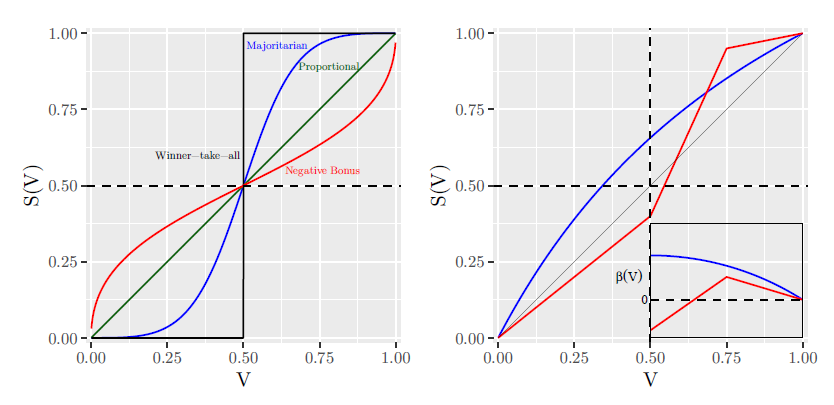
\includegraphics[width=\linewidth]{img/seatsvotes.png}
    \caption{Types of Seats-Votes Curves. Left panel: Symmetric (fair) curves with differing
    levels of electoral responsiveness. Right panel: Asymmetric (biased) curves, including
    one consistently biased toward the Democrats (blue) and one with biases favoring different
    parties depending on V (red); the inset graph is for (V ) for V 2 [0:5; 1] with the vertical
    axis scaled to be the same as the main plot, and lines color coded to the seats-votes curves. \parencite[175]{katz2020}}
    \label{fig:seatsvotes1}
\end{figure}

Partisan symmetry is usually observed by plotting a "seats-votes curve." This plot has $V$, the proportion of the overall votes won by the party, on the x-axis, and $S(V)$, the proportion of the seats won by the party, on the y-axis. Figure \ref{fig:seatsvotes1} \parencite[175]{katz2020} illustrates several hypothetical seats-votes curves.

Naturally, it's very rare to observe the necessary electoral outcomes under the same electoral system in order to determine partisan symmetry. (ie., it's very rare for two parties to tie one year, have one win 51\% of the total votes the next year, and then win 49\% of the votes the following year.)

In practice, one can estimate a seats-votes curve using the principle of uniform partisan swing.

\subsubsection{Uniform Partisan Swing}

Uniform partisan swing is the principle that when the overall vote share $V$ changes by some amount $dV$ between different elections under the same electoral system, the vote share at the district level also usually changes by the same $dV$. \textcite{katz2020} Empirically verified this to be true in 646 different elections. 

Thus, given a list of vote proportions per district ${v_1, v_2, v_3, ...}$ from one election, one can adjust each vote proportion by an arbitrarily small $dV$ until the seats share $S(V)$ is covered from 0 to 1. \parencite{katz2020}.

An example of such a curve is shown in Figure \ref{fig:seatsvotesups1}

\begin{figure}
    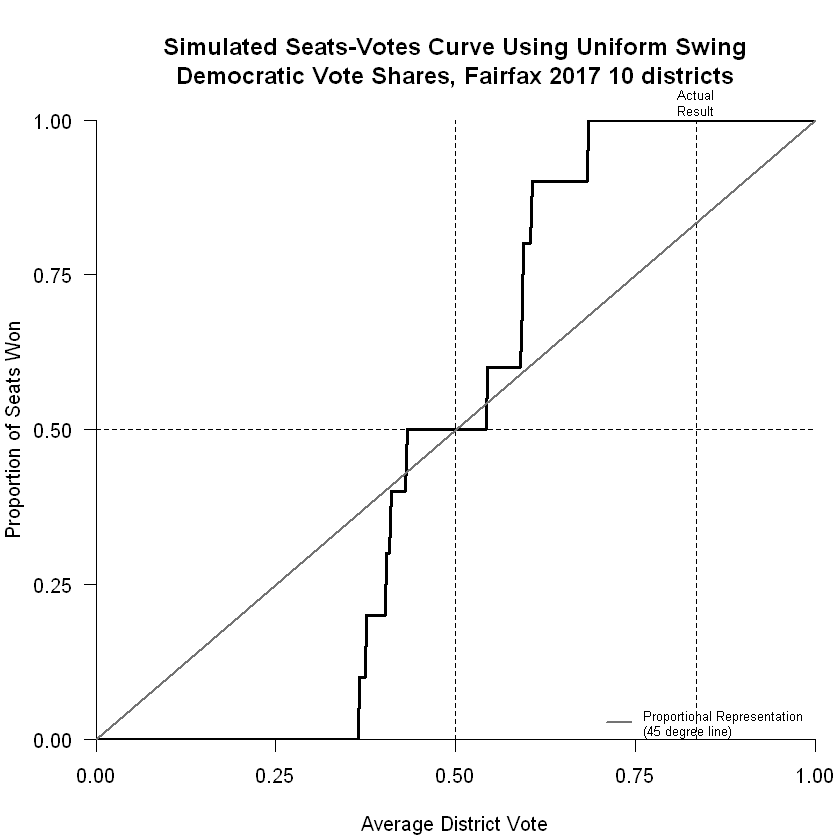
\includegraphics[width=0.5\linewidth]{img/seatsvotesups.png}
    \caption{Sample seats-votes curve generated using uniform partisan swing. Ignore title. \parencite[175]{katz2020}}
    \label{fig:seatsvotesups1}
\end{figure}

